\documentclass[]{book}
\usepackage{lmodern}
\usepackage{amssymb,amsmath}
\usepackage{ifxetex,ifluatex}
\usepackage{fixltx2e} % provides \textsubscript
\ifnum 0\ifxetex 1\fi\ifluatex 1\fi=0 % if pdftex
  \usepackage[T1]{fontenc}
  \usepackage[utf8]{inputenc}
\else % if luatex or xelatex
  \ifxetex
    \usepackage{mathspec}
  \else
    \usepackage{fontspec}
  \fi
  \defaultfontfeatures{Ligatures=TeX,Scale=MatchLowercase}
\fi
% use upquote if available, for straight quotes in verbatim environments
\IfFileExists{upquote.sty}{\usepackage{upquote}}{}
% use microtype if available
\IfFileExists{microtype.sty}{%
\usepackage{microtype}
\UseMicrotypeSet[protrusion]{basicmath} % disable protrusion for tt fonts
}{}
\usepackage{hyperref}
\hypersetup{unicode=true,
            pdftitle={All Models Are Wrong},
            pdfauthor={by Gaston Sanchez, and Ethan Marzban},
            pdfborder={0 0 0},
            breaklinks=true}
\urlstyle{same}  % don't use monospace font for urls
\usepackage{natbib}
\bibliographystyle{apalike}
\usepackage{longtable,booktabs}
\usepackage{graphicx,grffile}
\makeatletter
\def\maxwidth{\ifdim\Gin@nat@width>\linewidth\linewidth\else\Gin@nat@width\fi}
\def\maxheight{\ifdim\Gin@nat@height>\textheight\textheight\else\Gin@nat@height\fi}
\makeatother
% Scale images if necessary, so that they will not overflow the page
% margins by default, and it is still possible to overwrite the defaults
% using explicit options in \includegraphics[width, height, ...]{}
\setkeys{Gin}{width=\maxwidth,height=\maxheight,keepaspectratio}
\IfFileExists{parskip.sty}{%
\usepackage{parskip}
}{% else
\setlength{\parindent}{0pt}
\setlength{\parskip}{6pt plus 2pt minus 1pt}
}
\setlength{\emergencystretch}{3em}  % prevent overfull lines
\providecommand{\tightlist}{%
  \setlength{\itemsep}{0pt}\setlength{\parskip}{0pt}}
\setcounter{secnumdepth}{5}
% Redefines (sub)paragraphs to behave more like sections
\ifx\paragraph\undefined\else
\let\oldparagraph\paragraph
\renewcommand{\paragraph}[1]{\oldparagraph{#1}\mbox{}}
\fi
\ifx\subparagraph\undefined\else
\let\oldsubparagraph\subparagraph
\renewcommand{\subparagraph}[1]{\oldsubparagraph{#1}\mbox{}}
\fi

%%% Use protect on footnotes to avoid problems with footnotes in titles
\let\rmarkdownfootnote\footnote%
\def\footnote{\protect\rmarkdownfootnote}

%%% Change title format to be more compact
\usepackage{titling}

% Create subtitle command for use in maketitle
\providecommand{\subtitle}[1]{
  \posttitle{
    \begin{center}\large#1\end{center}
    }
}

\setlength{\droptitle}{-2em}

  \title{All Models Are Wrong}
    \pretitle{\vspace{\droptitle}\centering\huge}
  \posttitle{\par}
  \subtitle{Concepts of Statistical Learning (CSL)}
  \author{by Gaston Sanchez, and Ethan Marzban}
    \preauthor{\centering\large\emph}
  \postauthor{\par}
      \predate{\centering\large\emph}
  \postdate{\par}
    \date{2019-11-02}

\usepackage{booktabs}

\begin{document}
\maketitle

{
\setcounter{tocdepth}{1}
\tableofcontents
}
\hypertarget{part-welcome}{%
\part{Welcome}\label{part-welcome}}

\hypertarget{preface}{%
\chapter*{Preface}\label{preface}}
\addcontentsline{toc}{chapter}{Preface}

This is a work in progress for an introductory text about concepts of
Statistical Learning, covering common supervised as well as unsupervised methods.

\textbf{How to cite this book}:

Sanchez, G., Marzban E. (2019) \textbf{All Models Are Wrong: Concepts of Statistical Learning}.
\url{https://allmodelsarewrong.github.io}

© 2019 Sanchez, Marzban. All Rights Reserved.

\hypertarget{about}{%
\chapter{About this book}\label{about}}

Knowing that the field(s) of Machine Learning, Statisticial Learning, and any
other name about learning from data, is a very broad subject, we should warn you
that this book is not intended to be the ultimate compilation of every single
SL technique ever devised.

Instead, we focus on the concepts that we consider the building blocks that any
user or practitioner needs to make sense of most common SL techniques.

A big shortcoming of the book: we don't cover neural networks. At least not in this first round of iterations. Sorry!

On the plus side: We've tried hard to keep the notation as simple and consistent
as possible. And we've also made a serious effort to make it very visual
(lots of diagrams, pictures, plots, graphs, figures, \ldots, you name it).

\hypertarget{prerequisites}{%
\section{Prerequisites}\label{prerequisites}}

We are assuming that you already have some knowledge under your belt.

You will better understand (and hopefully enjoy) the book if you've taken one
or more courses on the following subjects:

\begin{itemize}
\tightlist
\item
  linear or matrix algebra
\item
  multivariable calculus
\item
  statistics
\item
  probability
\item
  programming or scripting
\end{itemize}

\hypertarget{acknowledgements}{%
\section{Acknowledgements}\label{acknowledgements}}

Many thanks to the UC Berkeley students of Stat 154 Modern Statistical Prediction
and Machine Learning (Fall 2017, Spring 2018, Fall 2019).

\hypertarget{part-intro}{%
\part{Intro}\label{part-intro}}

\hypertarget{intro}{%
\chapter{Introduction}\label{intro}}

Picture a data set containing scores of several course for college students.
For example, courses like matrix algebra, multivariable calculus,
statistics, and probability. And say we also have historical data about a course in Statistical
Learning. In particular we have final scores measured on a scale from 0 to 100,
we also have final grades (letter grade scale), as well as a third interesting
variable ``Pass - Non-Pass'' indicating whether the student passed statistical learning.
Some data like that fits perfectly well in a tabular format. The rows contain
the records for a bunch of students, and the columns refer to the variables.

\begin{longtable}[]{@{}lllllll@{}}
\toprule
Math 54 & Math 55 & Stat 135 & Stat 134 & Stat 154 & Grade & P/NP\tabularnewline
\midrule
\endhead
\(x_{11}\) & \(x_{12}\) & \(x_{13}\) & \(x_{14}\) & \(x_{15}\) & \(y_{15}\) & \(y_{16}\)\tabularnewline
\(x_{21}\) & \(x_{22}\) & \(x_{23}\) & \(x_{24}\) & \(x_{25}\) & \(y_{15}\) & \(y_{16}\)\tabularnewline
\ldots{} & \ldots{} & \ldots{} & \ldots{} & \ldots{} & \ldots{} & \ldots{}\tabularnewline
\(x_{n1}\) & \(x_{n2}\) & \(x_{n3}\) & \(x_{n4}\) & \(x_{n5}\) & \(y_{n5}\) & \(y_{n6}\)\tabularnewline
\bottomrule
\end{longtable}

Suppose that, based on this historical data, we wish to predict the score of a
new student (whose Math 54, Math 55, and Stat 135 grades are known) in Stat 154.

To do so, we would fit some sort of model to our data; i.e.~we would perform
regression. This is a form of supervised learning, since our model is trained
using known inputs (i.e.~Math 54, Math 55, and Stat 135 grades) as well as
known responses (i.e.~the Stat 154 grades of the previous students).

\textbf{Unsupervised Learning}: where we have inputs, but not response variables.

\hypertarget{basic-notation}{%
\section{Basic Notation}\label{basic-notation}}

In this book we are going to use a fair amount of math notation. Becoming familiar
with the meaning of all the different symbols as soon as possible, should allow
you to keep the learning curve a little bit less steep.

The starting point is always the data, which we will assume to be in a tabular
format, that can be translated into a mathematical matrix object. Here's an
example of a data matrix \(\mathbf{X}\) of size \(n \times p\)

\[
\mathbf{X} = 
\
\begin{bmatrix} 
x_{11} & x_{12} & \cdots & x_{1p} \\
x_{21} & x_{22} & \cdots & x_{2p} \\
\vdots & \vdots & \ddots & \vdots \\
x_{n1} & x_{n2} & \cdots & x_{np} \\
\end{bmatrix}
\]

By default, we will assume that the rows of a data matrix correspond to the
individuals or objects. Likewise, we will also assume that the columns of a data
matrix correspond to the variables or features observed on the individuals.
In this sense, the symbol \(x_{ij}\) represents the value observed for the \(j\)-th
variable on the \(i\)-th individual.

Throughout this book, every time you see the letter \(i\), either alone or as an
index associated with any other symbol (superscript or subscript), it means
that such term corresponds to an individual or a row of some data matrix.
For instance, symbols like \(x_i\), \(\mathbf{x_i}\), and \(\alpha_i\) are all
examples that refer to---or denote a connection with---individuals.

In turn, we will always use the letter \(j\) to conveyed association with variables.
For instance, \(x_j\), \(\mathbf{x_j}\), and \(\alpha_j\) are examples that refer
to---or denote a connection with---variables.

For better or for worse, we've made the decision to represent row vectors and column
vectors with the same notation: as bold lower case letters such as \(\mathbf{x_i}\) and
\(\mathbf{x_j}\). Because of the risk of confusing a row vector with a column vector,
sometimes we will use the arrow notation for row vectors: \(\mathbf{\vec{x}_i}\).

So, going back to the above data matrix \(\mathbf{X}\), we can represent the first
variable as a vector \(\mathbf{x_1} = (x_{11}, x_{21}, \dots, x_{n1})\).
Likewise, we can represent the first individual with the vector
\(\mathbf{\vec{x}_1} = (x_{11}, x_{12}, \dots, x_{1n})\).

Here's a reference table with the notation and symbols used throughout the book

\begin{longtable}[]{@{}ll@{}}
\toprule
Symbol & Description\tabularnewline
\midrule
\endhead
\(n\) & number of objects\tabularnewline
\(p\) & number of variables\tabularnewline
\(i\) & running index for rows\tabularnewline
\(j\) & running index for columns\tabularnewline
\(k\) & running index for sets of variables (i.e.~blocks)\tabularnewline
\(l, m, q\) & auxiliar index\tabularnewline
\(f()\), \(g()\), \(h()\) & functions\tabularnewline
\(\lambda, \mu, \gamma, \alpha\) & greek letters represent scalars\tabularnewline
\(\varepsilon\) & decimal tolerance threshold (e.g.~0.00001)\tabularnewline
\(\mathbf{x}\), \(\mathbf{y}\) & variables, size determined by context\tabularnewline
\(\mathbf{w}\), \(\mathbf{a}\), \(\mathbf{b}\) & vectors of weight coefficients\tabularnewline
\(\mathbf{z}\), \(\mathbf{t}\), \(\mathbf{u}\) & components or latent variables\tabularnewline
\(\mathbf{X} : n \times p\) & data matrix with \(n\) rows and \(p\) columns\tabularnewline
\(x_{ij}\) & element of a matrix in \(i\)-th row and \(j\)-th column\tabularnewline
\(\mathbf{1}\) & vector of ones, size determined by context\tabularnewline
\(\mathbf{I}\) & identity matrix, size determined by context\tabularnewline
\bottomrule
\end{longtable}

By the way, there are many more symbols that will appear in later chapters.
But for now these are the fundamental ones.

Common operators

\begin{longtable}[]{@{}ll@{}}
\toprule
Symbol & Description\tabularnewline
\midrule
\endhead
\(\mathbb{E}[X]\) & expected value of a random variable \(X\)\tabularnewline
\(\|\mathbf{a}\|\) & euclidean norm of a vector\tabularnewline
\(\mathbf{a}^{\mathsf{T}}\) & transpose of a vector (or matrix)\tabularnewline
\(\mathbf{a^{\mathsf{T}}b}\) & inner product of two vectors\tabularnewline
\(\langle \mathbf{a}, \mathbf{b} \rangle\) & inner product of two vectors\tabularnewline
\(det(\mathbf{A})\) & determinant of a square matrix\tabularnewline
\(tr(\mathbf{A})\) & trace of a square matrix\tabularnewline
\(\mathbf{A}^{-1}\) & inverse of a square matrix\tabularnewline
\(diag(\mathbf{A})\) & diagonal of a square matrix\tabularnewline
\(var()\) & variance\tabularnewline
\(cov()\) & covariance\tabularnewline
\bottomrule
\end{longtable}

\hypertarget{about-statistical-learning}{%
\section{About Statistical Learning}\label{about-statistical-learning}}

We will focus on supervised learning as well as unsupervised learning.
We won't discuss more recent fields of deep learning and reinforcement learning.

To visualize the different types of learning, the different types of variables, and the methodology associated with each combination of learning/data types, we can use the following graphic:

\begin{figure}

{\centering 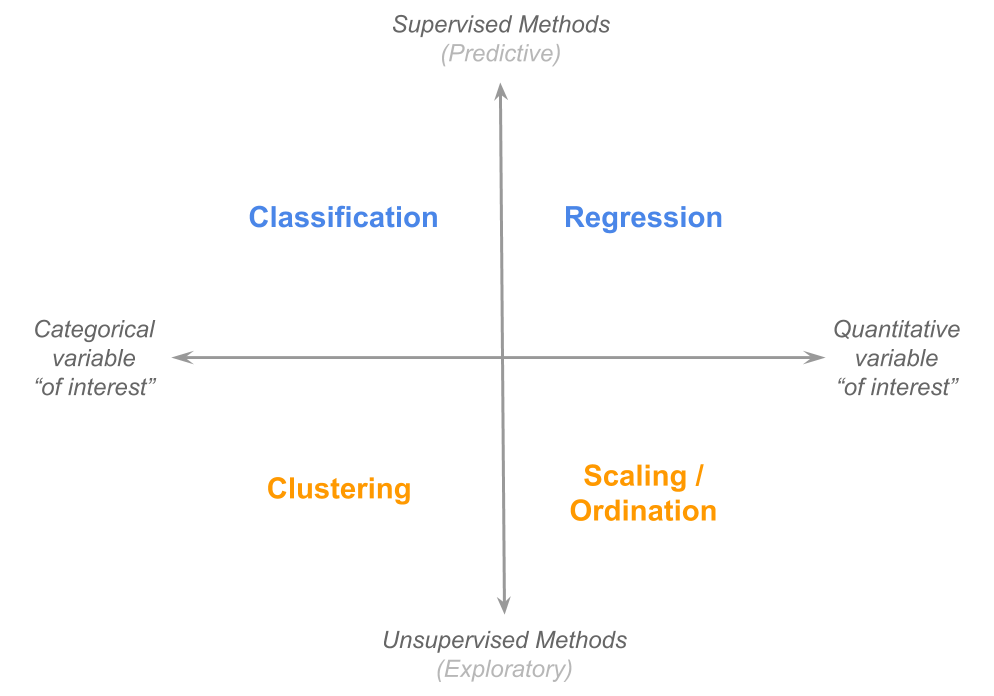
\includegraphics[width=0.8\linewidth]{images/introduction/four_corners} 

}

\caption{Supervised and Unsupervised}\label{fig:unnamed-chunk-5}
\end{figure}

\hypertarget{duality}{%
\chapter{Geometric Duality}\label{duality}}

The way we like to introduce you to the statistical learning world, is by
talking and thinking about data in a geometric sense.

Let's suppose we have some data in the form of a data matrix. For convenience
purposes, let's also suppose that all variables are measured in a real-value scale.
Obviously not all data is expressed or even encoded numerically. You may have
categorical or symbolic data. But for this illustration, let's assume that any
categorical and symbolic data has already been transformed into a numeric scale.

It's very enlightening to think of a data matrix as viewed from the glass of
Geometry. The key idea is to think of the data in a matrix as elements living
in a multidimensional space. Actually, we can regard a data matrix from two
apparently different perspectives that, in reality, are intimately connected:
the \textbf{rows perspective} and the \textbf{columns perspective}. In order to explain
these perspectives, let me use the following diagram of a data matrix \(\mathbf{X}\)
with \(n\) rows and \(p\) columns, with \(x_{ij}\) representing the element in the \(i\)-th
row and \(j\)-th column.

\begin{figure}

{\centering 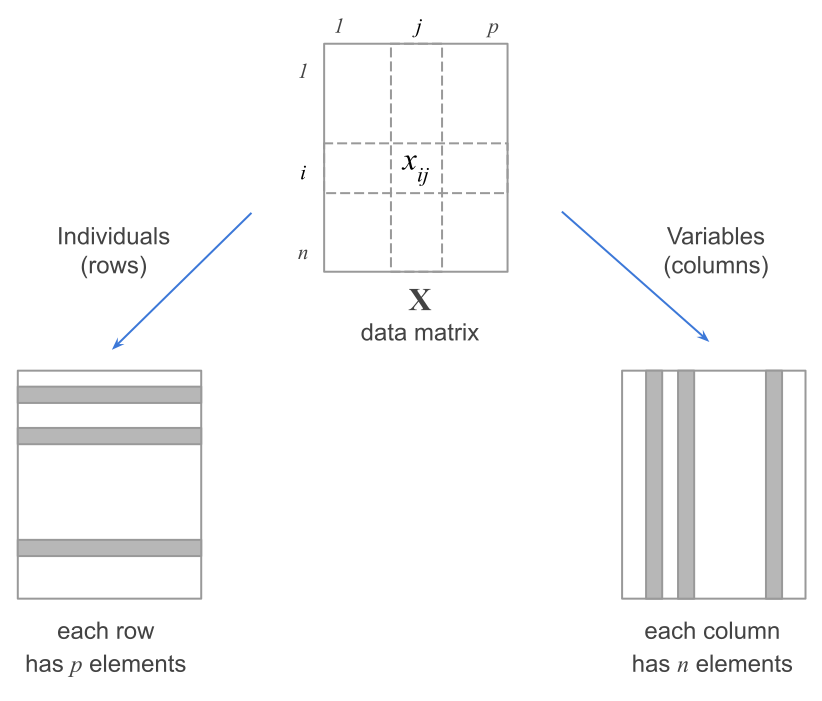
\includegraphics[width=0.7\linewidth]{images/duality/data-perspectives} 

}

\caption{Duality of a data matrix}\label{fig:unnamed-chunk-7}
\end{figure}

When we look at a data matrix from the \emph{columns} perpective what we are doing is focusing on the \(p\) variables. In a similar way, when looking at a data matrix from its \emph{rows} perspective, we are focusing on the \(n\) individuals.
Like a coin, though, this matrix has two sides: a rows side, and a columns side.
That is, we could look at the data from the rows point of view, or the columns
point of view. These two views are (of course) not completely independent.
This double perspective or \textbf{duality} for short, is like the two sides of the
same coin.

\hypertarget{rows-space}{%
\section{Rows Space}\label{rows-space}}

We know that human vision is limited to three-dimensions, but pretend that you had superpowers that let you visualize a space with any number of dimensions.

Because each row of the data matrix has \(p\) elements, we can regard individuals as objects that live in a \(p\)-dimensional space. For visualization purposes, think of each variable as playing the role of a dimension associated to a given axis in this space; likewise, consider each of the \(n\) individuals as being depicted as a point (or particle) in such space, like in the following diagram:

\begin{figure}

{\centering 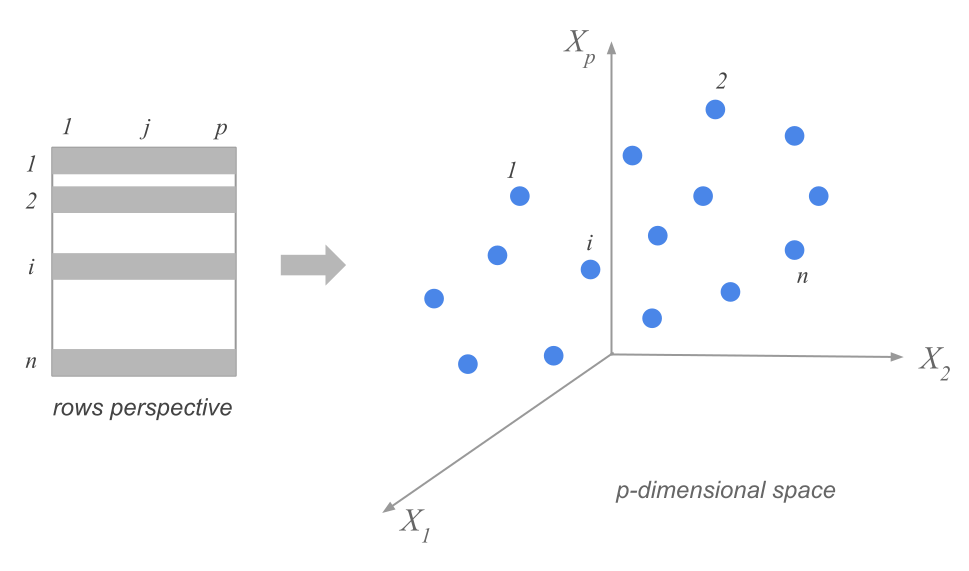
\includegraphics[width=0.85\linewidth]{images/duality/rows-space} 

}

\caption{Rows space}\label{fig:unnamed-chunk-8}
\end{figure}

In the figure above, even though I'm showing only three axes, you should pretend that you are visualizing a \(p\)-dimensional space (imaging that there are \(p\) axes). Each point in this space corresponds to a single individual, and they all form what you can call a \emph{cloud of points}.

\hypertarget{columns-space}{%
\section{Columns Space}\label{columns-space}}

We can do the same visual exercise with the columns of a data matrix. Since each variable has \(n\) elements, we can regard the set of \(p\) variables as objects that live in an \(n\)-dimensional space. However, instead of representing each variable with a dot, it's better to graphically represent them with an arrow (or vector). Why? Because of two reasons: one is to distinguish them from the individuals (dots). But more important, because the esential thing with a variable is not really its magnitude (and therefore its position) but its direction. Often, as part of the preprocessing steps we apply transformations on variables that change their scales (e.g.~shrinking them, or stretching them) without modifying their directions.

\begin{figure}

{\centering 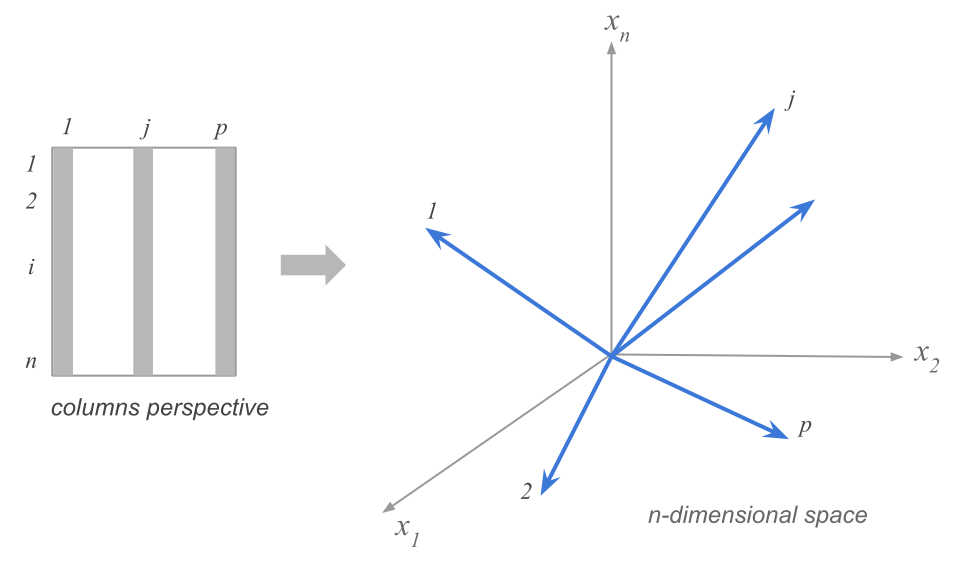
\includegraphics[width=0.85\linewidth]{images/duality/columns-space} 

}

\caption{Columns space}\label{fig:unnamed-chunk-9}
\end{figure}

Analogously to the rows space and its cloud of individuals, you should also
pretend that the image above is displaying an \(n\)-dimensional space with
a bunch of blue arrows pointing in various directions.

\hypertarget{whats-next}{%
\subsubsection*{What's next?}\label{whats-next}}
\addcontentsline{toc}{subsubsection}{What's next?}

Now that we know how to think of data from a geometric perspective, the next
step is to discuss a handful of common operations that can be performed with
points and vectors that live in some geometric space.

\begin{center}\rule{0.5\linewidth}{\linethickness}\end{center}

\hypertarget{cloud-of-individuals}{%
\section{Cloud of Individuals}\label{cloud-of-individuals}}

In the previous chapter we introduce the powerful idea of looking at the
rows and columns of a data matrix from the lens of geometry.
We are assuming in general that the rows have to do with \(n\) individuals that
lie in a \(p\)-dimensional space.

\begin{figure}

{\centering 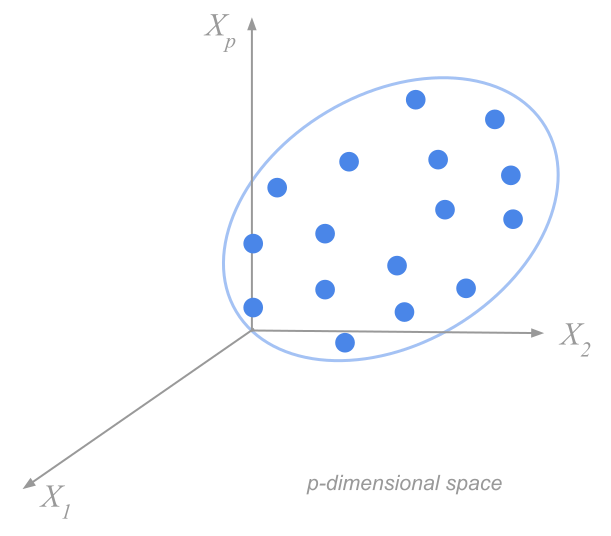
\includegraphics[width=0.55\linewidth]{images/duality/cloud-obs-centering0} 

}

\caption{Cloud of points}\label{fig:unnamed-chunk-10}
\end{figure}

Let's start describing a set of common operations that we can apply on the individuals
(living in a \(p\)-dimensional space).

\hypertarget{average-individual}{%
\subsection{Average Individual}\label{average-individual}}

We can ask about the typical or average individual.

If you only have one variable, then all the individual points lie in a one-dimensional space, which is basically a line:

\begin{figure}

{\centering 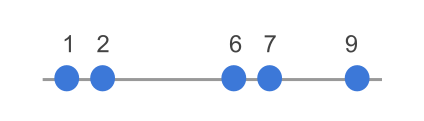
\includegraphics[width=0.3\linewidth]{images/duality/mean-number-line} 

}

\caption{Points in one dimension}\label{fig:unnamed-chunk-11}
\end{figure}

In this case, the average individual is simply the average of the values, which geometrically corresponds to the balancing point:

\begin{figure}

{\centering 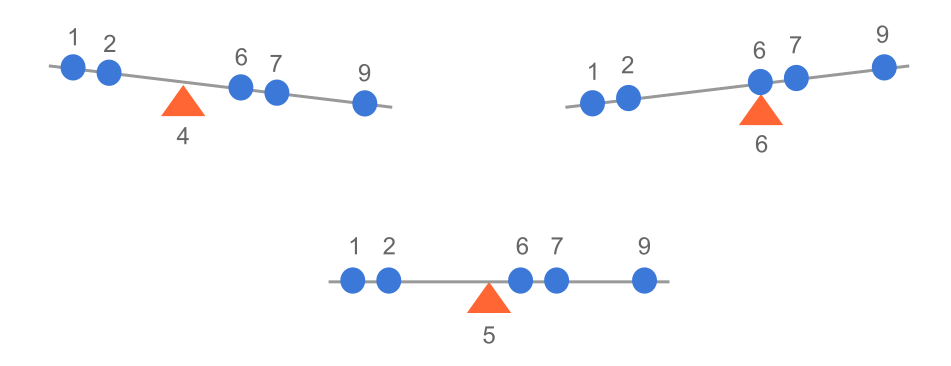
\includegraphics[width=0.7\linewidth]{images/duality/mean-balancing} 

}

\caption{Average individual}\label{fig:unnamed-chunk-12}
\end{figure}

Algebraically we have: individuals \(x_1, x_2, \dots, x_n\), and the average is:

\[
\bar{x} = \frac{x_1 + \dots + x_n}{n} = \frac{1}{n} \sum_{i=1}^{n} x_i
\]

In vector notation, the average can be calculated with an inner product between \(\mathbf{x} = (x_1, x_2, \dots, x_n)\), and a constant vector of \(n\)-ones \(\mathbf{1}\):

\[
\bar{x} = \mathbf{x^\mathsf{T}1}
\]

What about the multivariate case? It turns out that we can also ask about the average individual of a cloud of points, like in the following figure:

\begin{figure}

{\centering 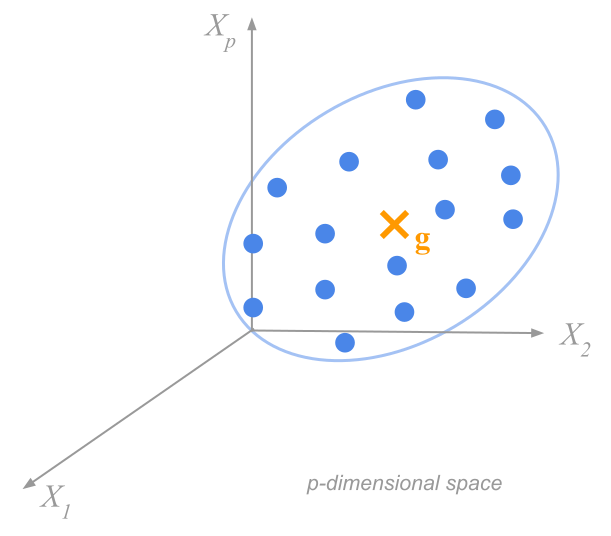
\includegraphics[width=0.55\linewidth]{images/duality/cloud-obs-centering1} 

}

\caption{Cloud of points with centroid (i.e. average individual)}\label{fig:unnamed-chunk-13}
\end{figure}

The average individual, in a \(p\)-dimensional space is the point \(\mathbf{\vec{g}}\)
containing as coordiantes the averages of all the variables:

\[
\mathbf{\vec{g}} = (\bar{x}_1, \bar{x}_2, \dots, \bar{x}_j)
\]

where \(\bar{x}_j\) is the average of the \(j\)-th variable.

This average individual \(\mathbf{\vec{g}}\) is also known as the \textbf{centroid}, \emph{barycenter}, or \emph{center of gravity} of the cloud of points.

\hypertarget{centered-data}{%
\subsection{Centered Data}\label{centered-data}}

Often, it is convenient to transform the data in such a way that the centroid of
a data set becomes the origin of the cloud of points. Geometrically, this type
of transformation involves a shif of the axes in the \(p\)-dimensional space.
Algebraically, this transformation corresponds to expresing the values of
each variable in terms of deviations from their means.

\begin{figure}

{\centering 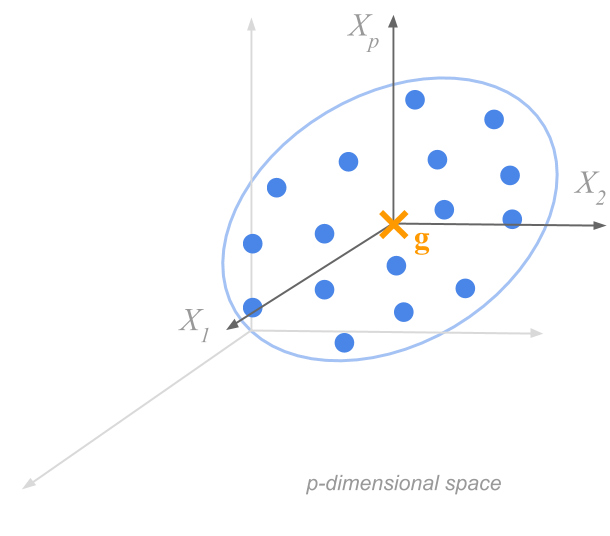
\includegraphics[width=0.55\linewidth]{images/duality/cloud-obs-centering2} 

}

\caption{Cloud of points of mean-centered data}\label{fig:unnamed-chunk-14}
\end{figure}

\hypertarget{distance-between-individuals}{%
\subsection{Distance between individuals}\label{distance-between-individuals}}

Another common operation that we may be interested in is the distance between two individuals. Obviously the notion of distance is not unique, since you can choose different types of distance measures. Perhaps the most comon type of distance is the (squared) Euclidean distance. Unless otherwise mentioned, this will be the default distance used in this book.

\begin{figure}

{\centering 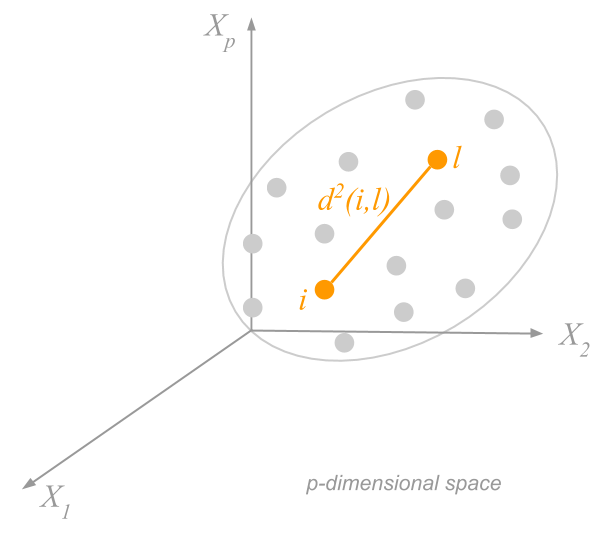
\includegraphics[width=0.55\linewidth]{images/duality/cloud-obs-distance} 

}

\caption{Distance between two individuals}\label{fig:unnamed-chunk-15}
\end{figure}

If you have one variable \(X\), then the squared distance \(d^2(i,l)\) between two individuals \(x_i\) and \(x_l\) is:

\[
d^2(i,l) = (x_i - x_l)^2
\]

In general, with \(p\) variables, the squared distance between the \(i\)-th individual
and the \(l\)-th individual is:

\begin{align*}
d^2(i,l) &= (x_{i1} - x_{l1})^2 + (x_{i2} - x_{l2})^2 + \dots + (x_{ip} - x_{lp})^2 \\
&= (\mathbf{\vec{x}_i} - \mathbf{\vec{x}_l})^\mathsf{T} (\mathbf{\vec{x}_i} - \mathbf{\vec{x}_l})
\end{align*}

\hypertarget{distance-to-the-centroid}{%
\subsection{Distance to the centroid}\label{distance-to-the-centroid}}

A special case is the distance between any individual \(i\) and the average individual:

\begin{align*}
d^2(i,g) &= (x_{i1} - \bar{x}_1)^2 + (x_{i2} - \bar{x}_2)^2 + \dots + (x_{ip} - \bar{x}_p)^2 \\
&= (\mathbf{\vec{x}_i} - \mathbf{\vec{g}})^\mathsf{T} (\mathbf{\vec{x}_i} - \mathbf{\vec{g}})
\end{align*}

\hypertarget{measures-of-dispersion}{%
\subsection{Measures of Dispersion}\label{measures-of-dispersion}}

What else can we calculate with the individuals? Think about it. So far we've
seen how to calculate the average individual, as well as distances between
individuals. The average individual or centroid plays the role of a measure
of center. And everytime you get a measure of center, it makes sense to get a
measure of spread.

\hypertarget{overall-dispersion}{%
\subsubsection*{Overall Dispersion}\label{overall-dispersion}}
\addcontentsline{toc}{subsubsection}{Overall Dispersion}

One way to compute a measure of scatter among individuals is to consider all the
squared distances between pairs of individuals. For instance, say you have three
individuals \(a\), \(b\), and \(c\). We can calculate all pairwise distances and add
them up:

\[
d^2(a,b) + d^2(b,a) + d^2(a,c) + d^2(c,a) + d^2(b,c) + d^2(c,b)
\]

In general, when you have \(n\) individuals, you can obtain up to \(n^2\) squared
distances. We will give the generic name of \textbf{Overall Dispersion} to the sum
of all squared pairwise distances:

\[
\text{overall dispersion} = \sum_{i=1}^{n} \sum_{l=1}^{n} d^2(i,l)
\]

\hypertarget{inertia}{%
\subsubsection*{Inertia}\label{inertia}}
\addcontentsline{toc}{subsubsection}{Inertia}

Another measure of scatter among individuals can be computed by adding the
distances between all individuals and the centroid.

\begin{figure}

{\centering 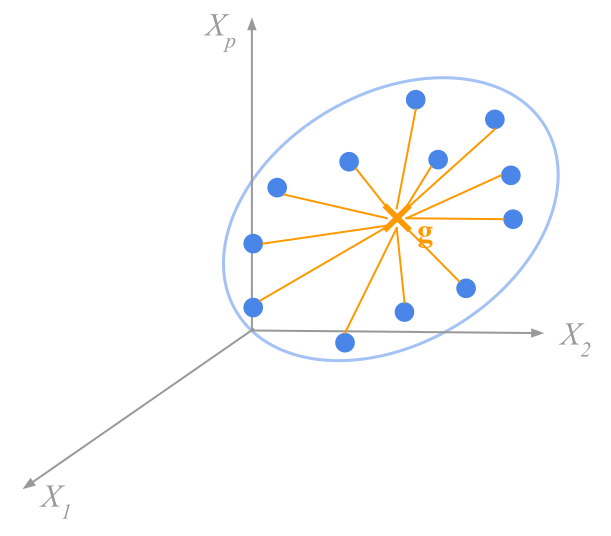
\includegraphics[width=0.55\linewidth]{images/duality/cloud-inertia} 

}

\caption{Inertia}\label{fig:unnamed-chunk-16}
\end{figure}

The sum of squared distances from each point to the centroid then becomes

\[
\frac{1}{n} \sum_{i=1}^{n} d^2(i,g) = \frac{1}{n} \sum_{i=1}^{n} (\mathbf{\vec{x}_i} - \mathbf{\vec{g}})^\mathsf{T} (\mathbf{\vec{x}_i} - \mathbf{\vec{g}})
\]

We will name this measure \textbf{Inertia}, borrowing this term from the concept of
inertia used in mechanics (in physics).

\[
\text{Inertia} = \frac{1}{n} \sum_{i=1}^{n} d^2(i,g)
\]

What is the motivation behind this measure? Consider the \(p = 1\) case; i.e.~
when \(\mathbf{X}\) is simply a column vector

\[
\mathbf{X} = \begin{pmatrix} x_1 \\ x_2 \\ \vdots \\ x_n \\ \end{pmatrix}
\]

The centroid will simply be the mean of these points: i.e.~
\(\bar{x} = \frac{1}{n} \sum_{i=1}^{n} x_i\).

The sum of squared-distances from each point to the centroid then becomes:

\[
(x_1 - \bar{x})^2 + (x_2 - \bar{x})^2 + \dots + (x_n - \bar{x})^2 = \sum_{i=1}^{n} (x_i - \bar{x})^2
\]

Does the above formula look familiar? What if we take the average of the squared distances:

\[
\frac{1}{n} \sum_{i=1}^{n} (x_i - \bar{x})^2 = \frac{(x_1 - \bar{x})^2 + (x_2 - \bar{x})^2 + \dots + (x_n - \bar{x})^2}{n}
\]

Same question: Do you recognize this formula? You better do\ldots{}
This is nothing else than the
formula of the variance of \(X\). And yes, we are dividing by \(n\) (not by \(n-1\)).
Hence, you can think of inertia as a multidimensional extension of variance,
which gives the typical squared distance around the centroid.

\hypertarget{overall-dispersion-and-inertia}{%
\subsubsection*{Overall Dispersion and Inertia}\label{overall-dispersion-and-inertia}}
\addcontentsline{toc}{subsubsection}{Overall Dispersion and Inertia}

Interestingly, the \emph{overall dispersion} and the \emph{inertia} are connected through
the following relation:

\begin{align*}
\text{overall dispersion} &= \sum_{i=1}^{n} \sum_{l=1}^{n} d^2(i,l) \\
&= 2n \sum_{i=1}^{n} d^2(i,g) \\
&= (2n^2) \text{Inertia}
\end{align*}

The proof of this relation is left as a homework exercise.

\begin{center}\rule{0.5\linewidth}{\linethickness}\end{center}

\hypertarget{cloud-of-variables}{%
\section{Cloud of Variables}\label{cloud-of-variables}}

The starting point when analyzing variables involves computing various summary
measures---such as means, and variances---to get an idea of the common or central
values, and the amount of variability of each variable. In this chapter we will
review how concepts like the mean of a variable, the variance, covariance,
and correlation, can be interpreted in a geometric sense, as well as their
expressions in terms of vector-matrix operations.

\hypertarget{mean-of-a-variable}{%
\subsection{Mean of a Variable}\label{mean-of-a-variable}}

To measure variation, we usually begin by calculating a ``typical'' value.
The idea is to summarize the values of a variable with one or two representative
values. You will find this notion under several terms like measures of center,
location, central tendency, or centrality.

The prototypical summary value of center is the \textbf{mean}, sometimes referred to
as average. The mean of an \(n-\)element variable \(X = (x_1, x_2, \dots, x_n)\),
represented by \(\bar{x}\), is obtained by adding all the \(x_i\) values and then
dividing by their total number \(n\):

\[
\bar{x} = \frac{x_1 + x_2 + \dots + x_n}{n}
\]

Using summation notation we can express \(\bar{x}\) in a very compact way as:

\[
\bar{x} = \frac{1}{n} \sum_{i = 1}^{n} x_i
\]

If you associate a constant weight of \(1/n\) to each observation \(x_i\), you can look at the formula of the mean as a weighted sum:

\[
\bar{x} = \frac{1}{n} x_1 + \frac{1}{n} x_2 + \dots + \frac{1}{n} x_n
\]

This is a slightly different way of looking at the mean that will allow you to
generalize the concept of an ``average'' as a \emph{weighted aggregation of information}.
For example, if we denote the weight of the \(i\)-th individual as \(w_i\), then the
average can be expressed as:

\[
\bar{x} = w_1 x_1 + w_2 x_2 + \dots + w_n x_n = \sum_{i=1}^{n} w_i x_i
\]

\hypertarget{variance-of-a-variable}{%
\subsection{Variance of a Variable}\label{variance-of-a-variable}}

A measure of center such as the mean is not enoguh to summarize the information
of a variable. We also need a measure of the amount of variability.
Synonym terms are variation, spread, scatter, and dispersion.

Because of its relevance and importance for statistical learning methods, we
will focus on one particular measure of spread: the \textbf{variance}
(and its square root the standard deviation).

Simply put, the variance is a measure of spread around the mean. The main idea
behind the calculation of the variance is to quantify the typical concentration
of values around the mean. The way this is done is by averaging the squared
deviations from the mean.

\[
var(X) = \frac{(x_1 - \bar{x})^2 + \dots + (x_n - \bar{x})^2}{n} = \frac{1}{n} \sum_{i=1}^{n} (x_i - \bar{x})^2
\]

Let's disect the terms and operations involved in the formula of the variance.

\begin{itemize}
\item
  the main terms are the \emph{deviations from the mean} \((x_i - \bar{x})\), that is, the difference between each observation \(x_i\) and the mean \(\bar{x}\).
\item
  conceptually speaking, we want to know what is the average size of the deviations around the mean.
\item
  simply averaging the deviations won't work because their sum is zero (i.e.~the sum of deviations around the mean will cancel out because the mean is the balancing point).
\item
  this is why we square each deviation: \((x_i - \bar{x})^2\), which literally means getting the squared distance from \(x_i\) to \(\bar{x}\).
\item
  having squared all the deviations, then we average them to get the variance.
\end{itemize}

Because the variance has squared units, we need to take the square root to
``recover'' the original units in which \(X\) is expressed.
This gives us the \textbf{standard deviation}

\[
sd(X) = \sqrt{\frac{1}{n} \sum_{i=1}^{n} (x_i - \bar{x})^2}
\]

In this sense, you can say that the standard deviation is roughly the average
distance that the data points vary from the mean.

\hypertarget{sample-variance}{%
\subsubsection*{Sample Variance}\label{sample-variance}}
\addcontentsline{toc}{subsubsection}{Sample Variance}

In practice, you will often find two versions of the formula for the variance:
one in which the sum of squared deviations is divided by \(n\), and another one
in which the division is done by \(n-1\). Each version is associated to the
statistical inference view of variance in terms of whether the data comes from
the \emph{population} or from a \emph{sample} of the population.

The \emph{population variance} is obtained dividing by \(n\):

\[
\textsf{population variance:} \quad \frac{1}{(n)} \sum_{i=1}^{n} (x_i - \bar{x})^2
\]

The \emph{sample variance} is obtained dividing by \(n - 1\) instead of dividing by \(n\).
The reason for doing this is to get an unbiased estimor of the population variance:

\[
\textsf{sample variance:} \quad \frac{1}{(n-1)} \sum_{i=1}^{n} (x_i - \bar{x})^2
\]

It is important to note that most statistical software compute the variance with
the unbiased version.
If you implement your own functions and are planning to compare them against
other software, then it is crucial to known what other programmers are using for
computing the variance. Otherwise, your results might be a bit different from
the ones with other people's code.

In this book, unless indicated otherwise, we will use the factor \(\frac{1}{n}\)
when introducing concepts of variance, and related measures. If needed, we will
let you know when a formula needs to use the factor \(\frac{1}{n-1}\).

\hypertarget{variance-with-vector-notation}{%
\subsection{Variance with Vector Notation}\label{variance-with-vector-notation}}

In a similar way to expressing the mean with vector notation, you can also
formulate the variance in terms of vector-matrix notation. First, notice that
the formula of the variance consists of the addition of squared terms.
Second, recall that a sum of numbers can be expressed with an inner product by
using the unit vector (or summation operator). If we denote a vector of ones of
size \(n\) as \(\mathbf{1}_{n}\), then the variance of a vector \(\mathbf{x}\) can be
obtained with the following inner product:

\[
var(\mathbf{x}) = \frac{1}{n} (\mathbf{x} - \mathbf{\bar{x}})^\mathsf{T} (\mathbf{x} - \mathbf{\bar{x}})
\]

where \(\mathbf{\bar{x}}\) is an \(n\)-element vector of mean values \(\bar{x}\).

Assuming that \(\mathbf{x}\) is already mean-centered, then the variance is
proportional to the squared norm of \(\mathbf{x}\)

\[
var(\mathbf{x}) = \frac{1}{n} \hspace{1mm} \mathbf{x}^{\mathsf{T}} \mathbf{x} = \frac{1}{n} \| \mathbf{x} \|^2
\]

This means that we can formulate the variance with the general notion of an
inner product:

\[
var(\mathbf{x}) = \frac{1}{n} \langle \mathbf{x}, \mathbf{x} \rangle
\]

\hypertarget{standard-deviation-as-a-norm}{%
\subsection{Standard Deviation as a Norm}\label{standard-deviation-as-a-norm}}

If we use a metric matrix \(\mathbf{D} = diag(1/n)\) then we have that the variance
is given by a special type of inner product:

\[
var(\mathbf{x}) = \langle \mathbf{x}, \mathbf{x} \rangle_{D} = \mathbf{x}^{\mathsf{T}} \mathbf{D x}
\]

From this point of view, we can say that the variance of \(\mathbf{x}\) is
equivalent to its squared norm when the vector space is endowed with a metric
\(\mathbf{D}\). Consequently, the standard deviation is simply the length of
\(\mathbf{x}\) in this particular geometric space.

\[
sd(\mathbf{x}) = \| \mathbf{x} \|_{D}
\]

When looking at the standard deviation from this perspective, you can actually
say that the amount of spread of a vector \(\mathbf{x}\) is actually its length
(under the metric \(\mathbf{D}\)).

\hypertarget{covariance}{%
\subsection{Covariance}\label{covariance}}

The covariance generalizes the concept of variance for two variables. Recall that the formula for the covariance between \(\mathbf{x}\) and \(\mathbf{y}\) is:

\[
cov(\mathbf{x, y}) = \frac{1}{n} \sum_{i=1}^{n} (x_i - \bar{x}) (y_i - \bar{y})
\]

where \(\bar{x}\) is the mean value of \(\mathbf{x}\) obtained as:

\[
\bar{x} = \frac{1}{n} (x_1 + x_2 + \dots + x_n) = \frac{1}{n} \sum_{i = 1}^{n} x_i
\]

and \(\bar{y}\) is the mean value of \(\mathbf{y}\):

\[
\bar{y} = \frac{1}{n} (y_1 + y_2 + \dots + y_n) = \frac{1}{n} \sum_{i = 1}^{n} y_i
\]

Basically, the covariance is a statistical summary that is used to assess the
\textbf{linear association between pairs of variables}.

Assuming that the variables are mean-centered, we can get a more compact
expression of the covariance in vector notation:

\[
cov(\mathbf{x, y}) = \frac{1}{n} (\mathbf{x^{\mathsf{T}} y})
\]

Properties of covariance:

\begin{itemize}
\tightlist
\item
  the covariance is a symmetric index: \(cov(X,Y) = cov(Y,X)\)
\item
  the covariance can take any real value (negative, null, positive)
\item
  the covariance is linked to variances under the name of the Cauchy-Schwarz inequality:
  \[cov(X,Y)^2 \leq var(X) var(Y) \]
\end{itemize}

\hypertarget{correlation}{%
\subsection{Correlation}\label{correlation}}

Although the covariance indicates the direction---positive or negative---of a possible linear relation, it does not tell us how big or small the relation might be. To have a more interpretable index, we must transform the convariance into a unit-free measure. To do this we must consider the standard deviations of the variables so we can normalize the covariance. The result of this normalization is the coefficient of linear correlation defined as:

\[
cor(X, Y) = \frac{cov(X, Y)}{\sqrt{var(X)} \sqrt{var(Y)}}
\]

Representing \(X\) and \(Y\) as vectors \(\mathbf{x}\) and \(\mathbf{y}\), we can express the correlation as:

\[
cor(\mathbf{x}, \mathbf{y}) = \frac{cov(\mathbf{x}, \mathbf{y})}{\sqrt{var(\mathbf{x})} \sqrt{var(\mathbf{y})}}
\]

Assuming that \(\mathbf{x}\) and \(\mathbf{y}\) are mean-centered, we can express the correlation as:

\[
cor(\mathbf{x, y}) = \frac{\mathbf{x^{\mathsf{T}} y}}{\|\mathbf{x}\| \|\mathbf{y}\|}
\]

As it turns out, the norm of a mean-centered variable \(\mathbf{x}\) is
proportional to the square root of its variance (or standard deviation):

\[
\| \mathbf{x} \| = \sqrt{\mathbf{x^{\mathsf{T}} x}} 
 = \sqrt{n} \sqrt{var(\mathbf{x})}
\]

Consequently, we can also express the correlation with inner products as:

\[
cor(\mathbf{x, y}) = \frac{\mathbf{x^{\mathsf{T}} y}}{\sqrt{(\mathbf{x^{\mathsf{T}} x})} \sqrt{(\mathbf{y^{\mathsf{T}} y})}}
\]

or equivalently:

\[
cor(\mathbf{x, y}) = \frac{\mathbf{x^{\mathsf{T}} y}}{\| \mathbf{x} \| \hspace{1mm} \| \mathbf{y} \|}
\]

In the case that both \(\mathbf{x}\) and \(\mathbf{y}\) are standardized (mean zero
and unit variance), that is:

\[
\mathbf{x} = \begin{bmatrix}
\frac{x_1 - \bar{x}}{\sigma_{x}} \\
\frac{x_2 - \bar{x}}{\sigma_{x}} \\
\vdots \\
\frac{x_n - \bar{x}}{\sigma_{x}}
\end{bmatrix},
\hspace{5mm}
\mathbf{y} = \begin{bmatrix}
\frac{y_1 - \bar{y}}{\sigma_{y}} \\
\frac{y_2 - \bar{y}}{\sigma_{y}} \\
\vdots \\
\frac{y_n - \bar{y}}{\sigma_{y}}
\end{bmatrix}
\]

the correlation is simply the inner product:

\[
cor(\mathbf{x, y}) = \mathbf{x^{\mathsf{T}} y} \hspace{5mm} \textsf{(standardized variables)}
\]

\hypertarget{geometry-of-correlation}{%
\subsection{Geometry of Correlation}\label{geometry-of-correlation}}

Let's look at two variables (i.e.~vectors) from a geometric perspective.

\begin{figure}

{\centering 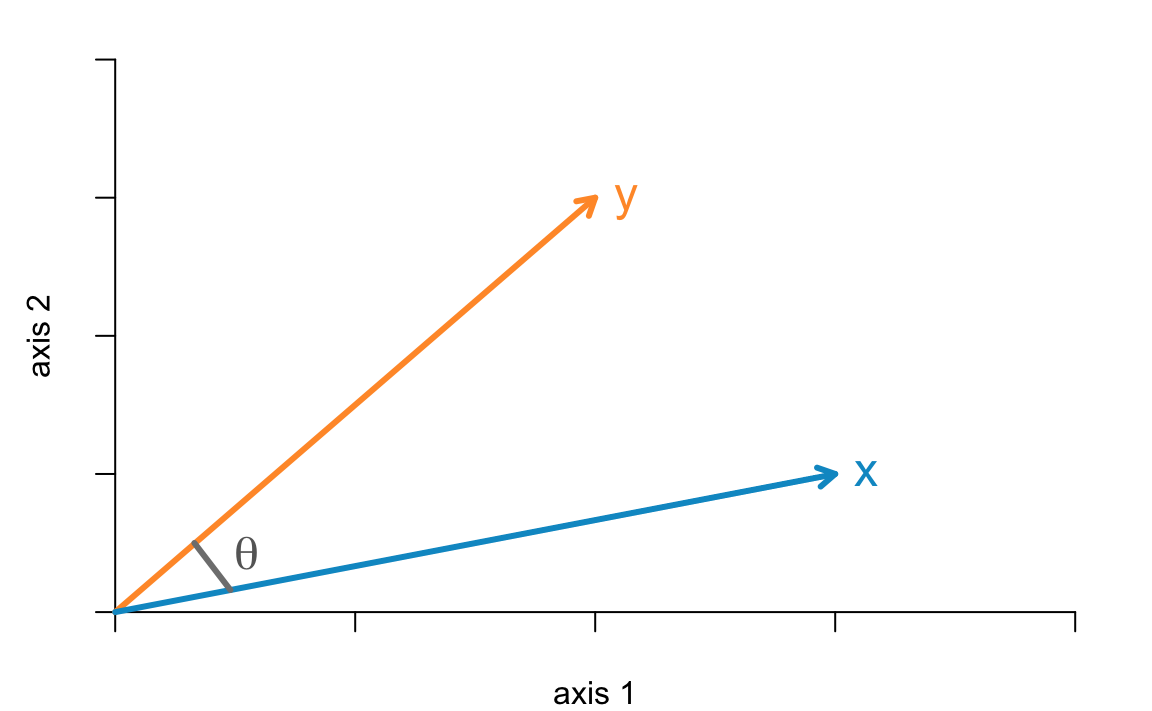
\includegraphics[width=0.7\linewidth]{allmodelsarewrong_files/figure-latex/unnamed-chunk-17-1} 

}

\caption{Two vectors in a 2-dimensional space}\label{fig:unnamed-chunk-17}
\end{figure}

The inner product ot two mean-centered vectors \(\langle \mathbf{x}, \mathbf{y} \rangle\) is obtained with the following equation:

\[
\mathbf{x^{\mathsf{T}} y} = \|\mathbf{x}\| \hspace{1mm} \|\mathbf{y}\| \hspace{1mm} cos(\theta_{x,y})
\]

where \(cos(\theta_{x,y})\) is the angle between \(\mathbf{x}\) and \(\mathbf{y}\). Rearranging the terms in the previous equation we get that:

\[
cos(\theta_{x,y}) = \frac{\mathbf{x^\mathsf{T} y}}{\|\mathbf{x}\| \|\mathbf{y}\|} = cor(\mathbf{x, y}) 
\]

which means that the correlation between mean-centered vectors \(\mathbf{x}\) and \(\mathbf{y}\) turns out to be the cosine of the angle between \(\mathbf{x}\) and \(\mathbf{y}\).

\hypertarget{orthogonal-projections}{%
\subsection{Orthogonal Projections}\label{orthogonal-projections}}

Last but not least, we finish this chapter with a discussion of projections.
To be more specific, the statistical interpretation of orthogonal projections.

Let's motivate this discussion with the following question: Consider two
variables \(\mathbf{x}\) and \(\mathbf{y}\). Can we approximate one of the variables
in terms of the other? This is
an asymmetric type of association since we seek to say something about the
variability of one variable, say \(\mathbf{y}\), in terms of the variability of
\(\mathbf{x}\).

\begin{figure}

{\centering 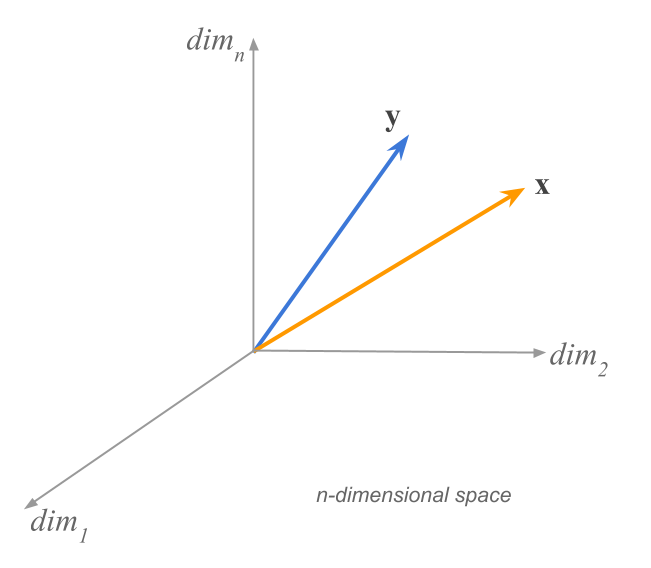
\includegraphics[width=0.6\linewidth]{images/duality/vector-projection0} 

}

\caption{Two vectors in n-dimensional space}\label{fig:unnamed-chunk-18}
\end{figure}

We can think of several ways to approximate \(\mathbf{y}\) in terms of
\(\mathbf{x}\). The approximation of \(\mathbf{y}\), denoted by \(\mathbf{\hat{y}}\),
means finding a scalar \(b\) such that:

\[
\mathbf{\hat{y}} = b \mathbf{x}
\]

The common approach to get \(\mathbf{\hat{y}}\) in some optimal way is by
minimizing the square difference between \(\mathbf{y}\) and \(\mathbf{\hat{y}}\).

\begin{figure}

{\centering 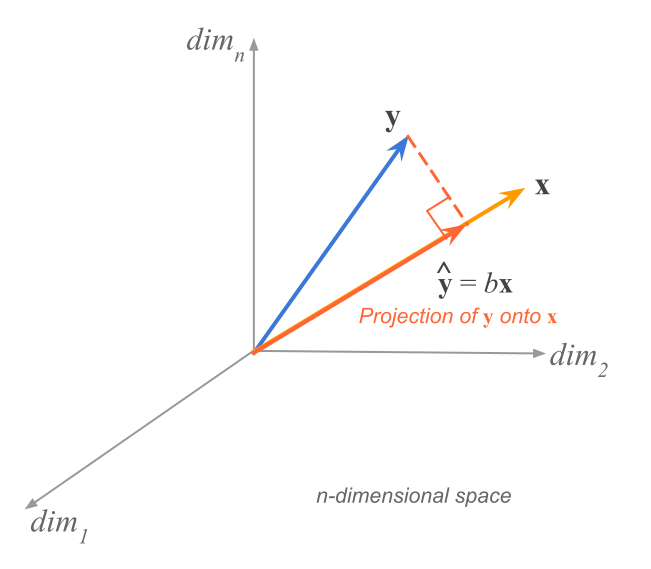
\includegraphics[width=0.6\linewidth]{images/duality/vector-projection1} 

}

\caption{Orthogonal projection of y onto x}\label{fig:unnamed-chunk-19}
\end{figure}

The answer to this question comes in the form of a projection. More precisely,
we orthogonally project \(\mathbf{y}\) onto \(\mathbf{x}\):

\[
\mathbf{\hat{y}} = \mathbf{x} \left( \frac{\mathbf{y^\mathsf{T} x}}{\mathbf{x^\mathsf{T} x}} \right)
\]

or equivalently:

\[
\mathbf{\hat{y}} = \mathbf{x} \left( \frac{\mathbf{y^\mathsf{T} x}}{\| \mathbf{x} \|^2} \right)
\]

For convenience purposes, we can rewrite the above equation in a slightly different
format:

\[
\mathbf{\hat{y}} = \mathbf{x} (\mathbf{x^\mathsf{T}x})^{-1} \mathbf{x^\mathsf{T}y}
\]

If you are familiar with linear regression, you should be able to recognize
this equation. We'll come back to this when we get to the chapter about
\protect\hyperlink{ols}{Linear regression}.

\hypertarget{the-mean-as-an-orthogonal-projection}{%
\subsection{The mean as an orthogonal projection}\label{the-mean-as-an-orthogonal-projection}}

Let's go back to the concept of mean of a variable. As we previously mention,
a variable \(X = (x_1, \dots, x_n)\), can be thought of a vector \(\mathbf{x}\)
in an \(n\)-dimensional space. Furthermore, let's also consider the constant
vector \(\mathbf{1}\) of size \(n\). Here's a conceptual diagram for this situation:

\begin{figure}

{\centering 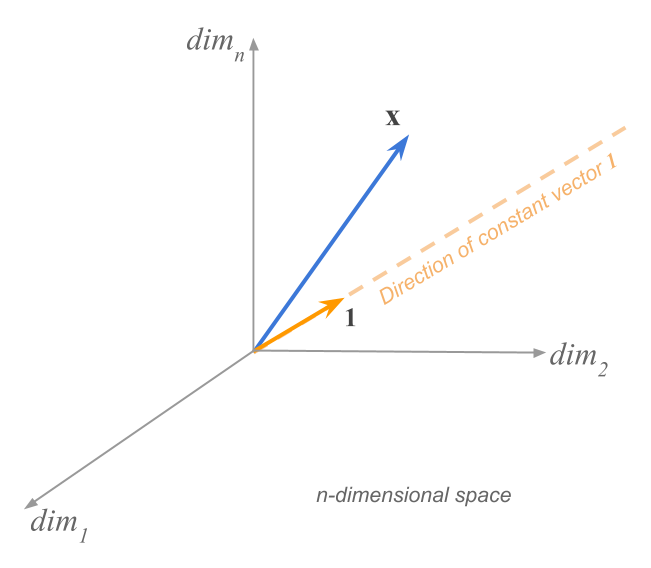
\includegraphics[width=0.6\linewidth]{images/duality/mean-projection0} 

}

\caption{Two vectors in n-dimensional space}\label{fig:unnamed-chunk-20}
\end{figure}

Out of curiosity, what happens when we ask about the orthogonal projection of
\(\mathbf{x}\) onto \(\mathbf{1}\)? Something like in the following picture:

\begin{figure}

{\centering 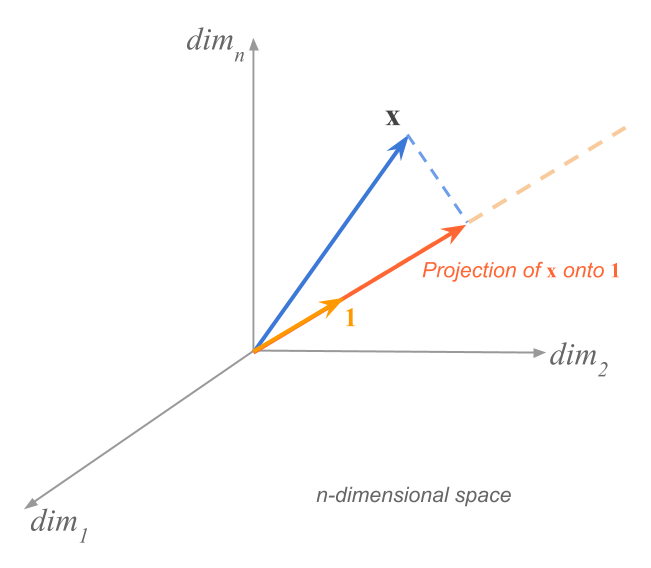
\includegraphics[width=0.6\linewidth]{images/duality/mean-projection1} 

}

\caption{Orthogonal projection of vector x onto constant vector 1}\label{fig:unnamed-chunk-21}
\end{figure}

This projection is expressed in vector notation as:

\[
\mathbf{\hat{x}} = \mathbf{1} \left( \frac{\mathbf{x^\mathsf{T} 1}}{\mathbf{1^\mathsf{T} 1}} \right)
\]

or equivalently:

\[
\mathbf{\hat{x}} = \mathbf{1} \left( \frac{\mathbf{x^\mathsf{T} 1}}{\| \mathbf{1} \|^2} \right)
\]

Note that the term in parenthesis is just a scalar, so we can actually express
\(\mathbf{\hat{x}}\) as \(b \mathbf{1}\). This means that a projection implies
multiplying \(\mathbf{1}\) by some number \(b\), such that
\(\mathbf{\hat{x}} = b \mathbf{1}\) is a stretched or shrinked version of
\(\mathbf{1}\). So, what is the scalar \(b\)? It is simply the mean of \(\mathbf{x}\):

\[
\mathbf{\hat{x}} = \mathbf{1} \left( \frac{\mathbf{x^\mathsf{T} 1}}{\| \mathbf{1} \|^2} \right) = \bar{x} \mathbf{1}
\]

This is better appreciated in the following figure.

\begin{figure}

{\centering 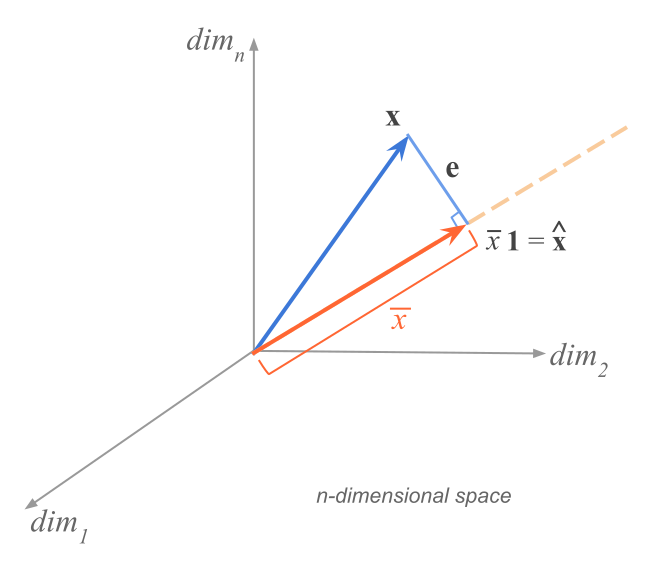
\includegraphics[width=0.6\linewidth]{images/duality/mean-projection2} 

}

\caption{Mean of x as length of its projection onto constant vector 1}\label{fig:unnamed-chunk-22}
\end{figure}

What this tells us is that the mean of the variable \(X\), denoted by \(\bar{x}\),
has a very interesting geometric interpretation. As you can tell, \(\bar{x}\) is
the length of the projected vector \(\mathbf{\hat{x}}\). Or in more formal terms,
\(\bar{x}\) is the scalar projection of \(\mathbf{x}\) onto \(\mathbf{1}\).

\hypertarget{part-unsupervised-i-pca}{%
\part{Unsupervised I: PCA}\label{part-unsupervised-i-pca}}

\hypertarget{pca}{%
\chapter{Principal Components Analysis}\label{pca}}

Our first unsupervised method of the book is Principal Components Analysis,
commonly referred to as PCA.

Principal Components Analysis (PCA) is the workhorse method of multivariate data
analysis. Simply put, PCA helps us study and explore a data set of quantitative
variables measured on a set of objects. One way to look at the purpose of principal
components analysis is to get the \emph{best} low-dimensional representation of the
variation in data. Among the various appealing features of PCA is that it allows
us to obtain a visualization of the objects in order to see their proximities.
Likewise, it also provides us results to get a graphic representation of the
variables in terms of their correlations. Overall, PCA is a multivariate technique
that allows us to summarize the systematic patterns of variations in a data set.

The classic reference for PCA is the work by the eminent British biostatistician
Karl Pearson ``On Lines and Planes of Closest Fit to Systems of Points in Space,''
from 1901. This publication presents the PCA problem under a purely geometric
standpoint, describing how to find low-dimensional subspaces that best
fit---in the least squares sense---a cloud of points. The other seminal work of
PCA is the one by the American mathematician and economic theorist Harold Hotelling
with ``Analysis of a Complex of Statistical Variables into Principal Components,''
from 1933. Unlike Pearson, Hotelling finds the principal components as
orthogonal linear combinations of the variables of maximum variance.

PCA is one of those methods that can be approached from multiple, seemingly
unrelated, perspectives. The way we are going to introduce PCA is not the typical
way in which PCA is discussed in most books published in English. However, our
introduction is actually based on the ideas and concepts originally published
in \href{https://en.wikipedia.org/wiki/Karl_Pearson}{Karl Pearson's} 1901 paper
\emph{On lines and planes of closest fit to systems of points in space}. This is what
can be considered to be the first paper on PCA, although keep in mind that
Karl Pearson never used the term \emph{principal components analysis}. That term was
coined by Harold Hotelling, who formalized the method by giving it a more
mature statistical perspective.

\hypertarget{low-dimensional-representations}{%
\section{Low-dimensional Representations}\label{low-dimensional-representations}}

Let's play the following game. Imagine for a minute that you have the superpower
to see any type of multidimensional space (not just three-dimensions). As we
mentioned before, we think of the individuals as forming a cloud of points in a
\(p\)-dim space, and the variables forming a cloud of arrows in an \(n\)-dim space.

Pretend that you have some data in which its cloud of points has the shape of
a mug, like in the following diagram:

\begin{figure}

{\centering 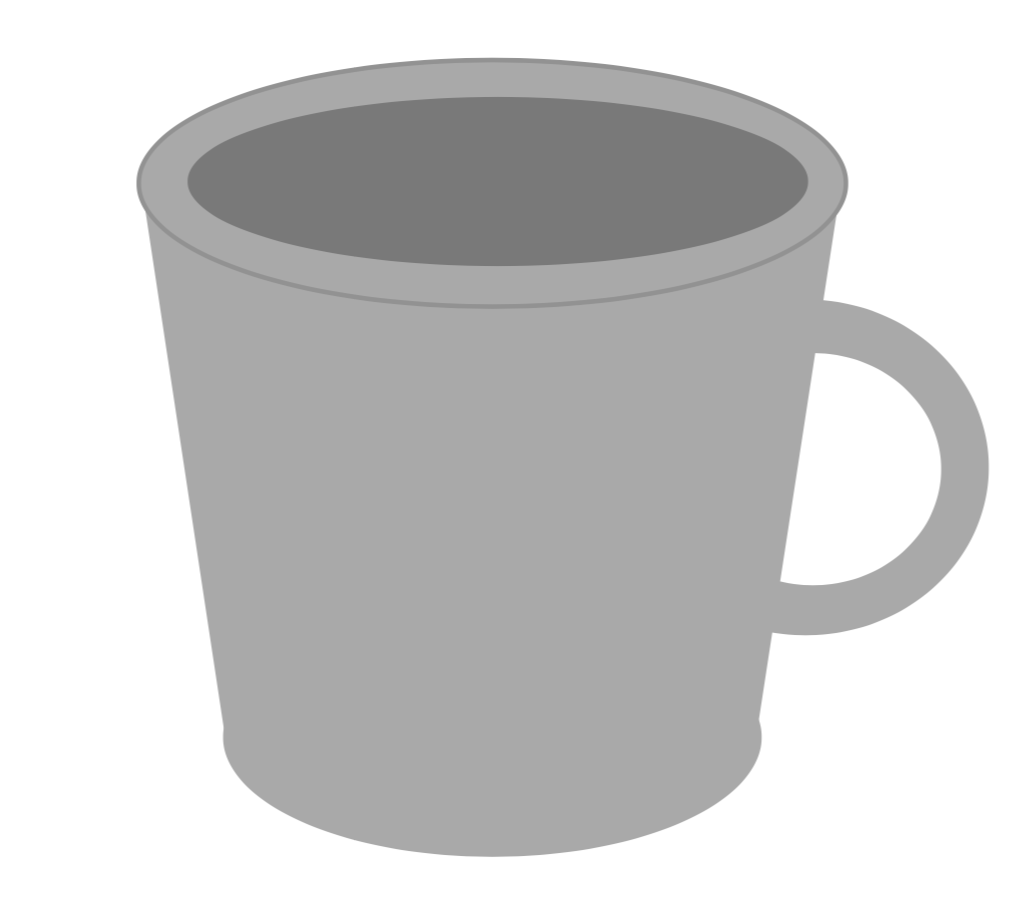
\includegraphics[width=0.4\linewidth]{images/pca/mug-data} 

}

\caption{Cloud of points in the form of a mug}\label{fig:unnamed-chunk-24}
\end{figure}

This mug is supposed be high-dimensional, and something that you are not supposed
to ever see in real life. So the question is: Is there a way in which we can get
a low-dimensional representation of this data?

Luckily, the answer is: YES, we can!

How? Well, the name of the game is \textbf{projections}: we can look for projections
of the data into sub-spaces of lower dimension, like in the diagram below.

\begin{figure}

{\centering 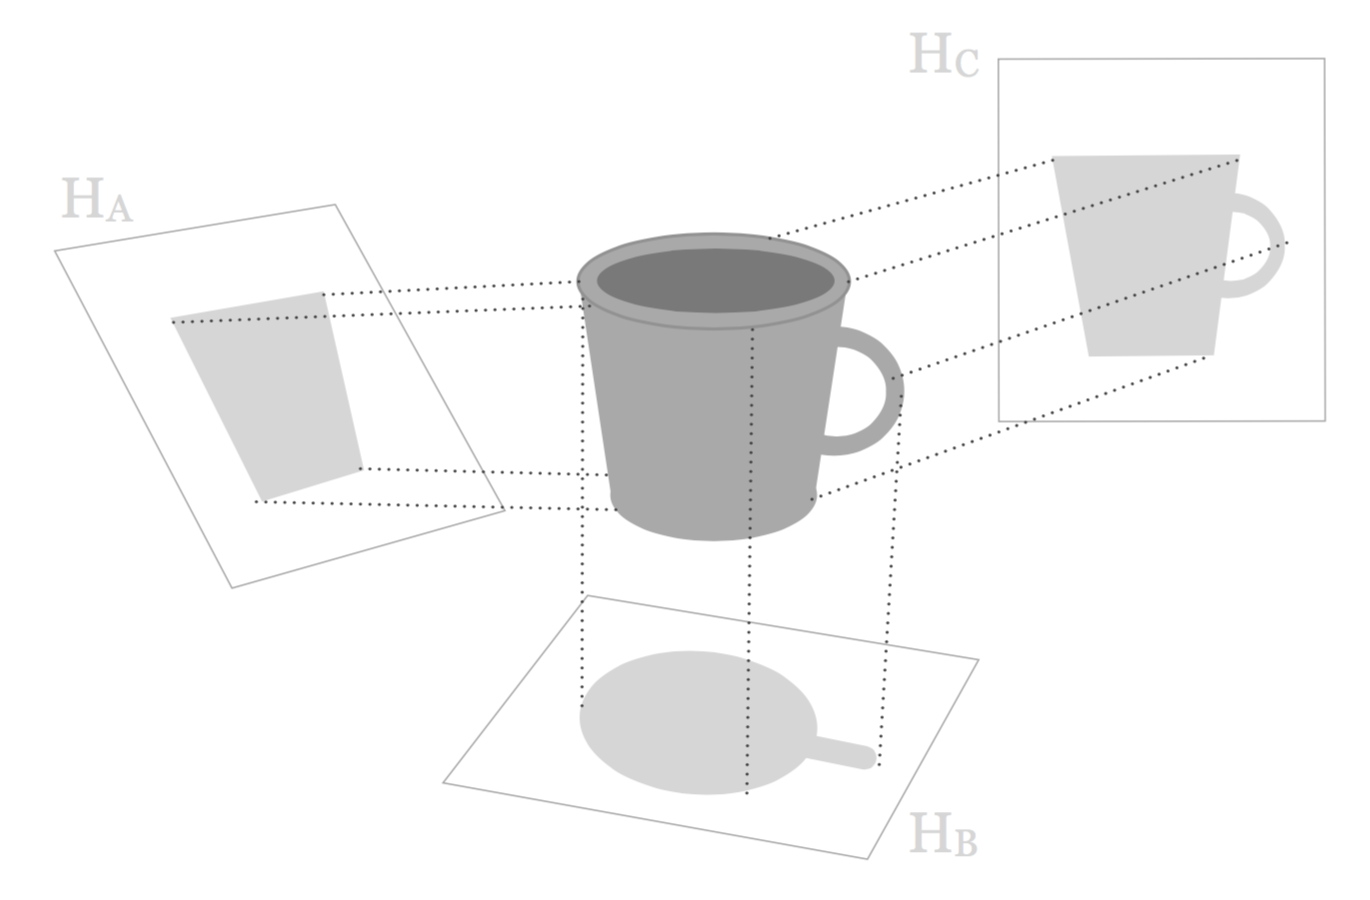
\includegraphics[width=0.7\linewidth]{images/pca/mug-projections} 

}

\caption{Various projections onto subspaces}\label{fig:unnamed-chunk-25}
\end{figure}

Think of \emph{projections} as taking photographs or x-rays of the mug. You can take a
photo of the mug from different angles. For instance, a picture in which the lens
of the camera lies on the top of the mug, or another picture in which the lens is
below the mug (from the bottom), and so on.

As you can tell from the above figure, we have three candidate subspaces:
\(\mathbb{H}_A\), \(\mathbb{H}_B\), and \(\mathbb{H}_C\). Among the three possible
projections, subspace \(\mathbb{H}_C\) is the one that provides the best low
dimensional representation, in the sense that the projected silhouette is the
most similar to the original mug shape. We can say that this ``photo'' is the one
that most resembles the original object. Now, keep in mind that the resulting
image in the low-dimensional space is not capturing the whole pattern. In other
words, there is some loss of information. However, by chosing the right project,
we hope to minimize such loss.

\begin{figure}

{\centering 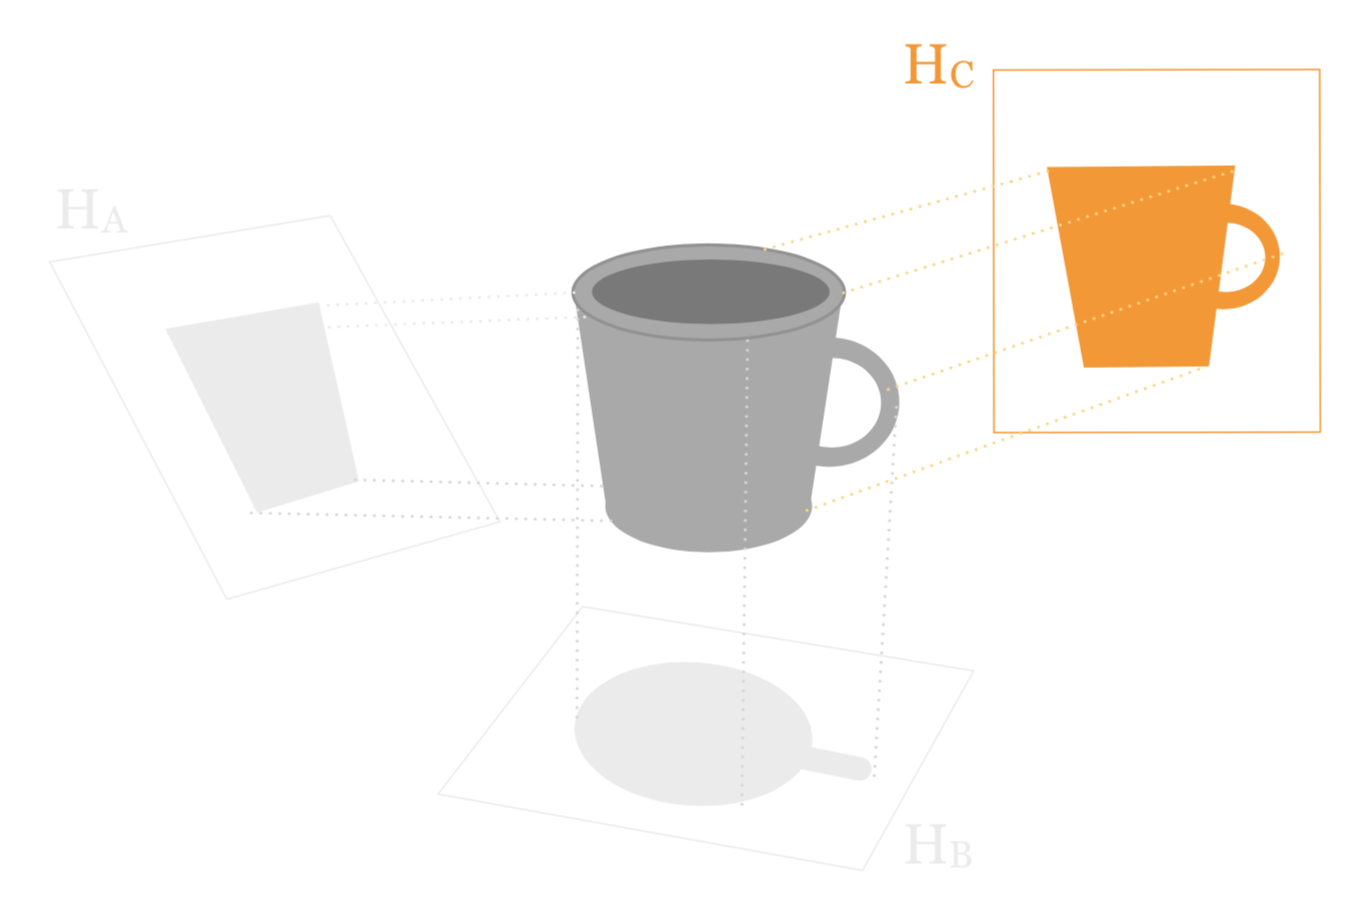
\includegraphics[width=0.5\linewidth]{images/pca/mug-subspace} 

}

\caption{The shape of the projection is similar to the original mug shape.}\label{fig:unnamed-chunk-26}
\end{figure}

\hypertarget{pca-idea}{%
\section{PCA Idea}\label{pca-idea}}

The overall idea behind PCA is the following. Given a set of \(p\) variables
\(\mathbf{x_1}, \mathbf{x_2}, \dots, \mathbf{x_p}\), we want to obtain new \(k\) variables
\(\mathbf{z_1}, \mathbf{z_2}, \dots, \mathbf{z_k}\), called the \textbf{Principal Components} (PCs).

A principal component is a linear combination: \(\mathbf{z} = \mathbf{Xv}\).
The first PC is a linear mix:

\begin{figure}

{\centering 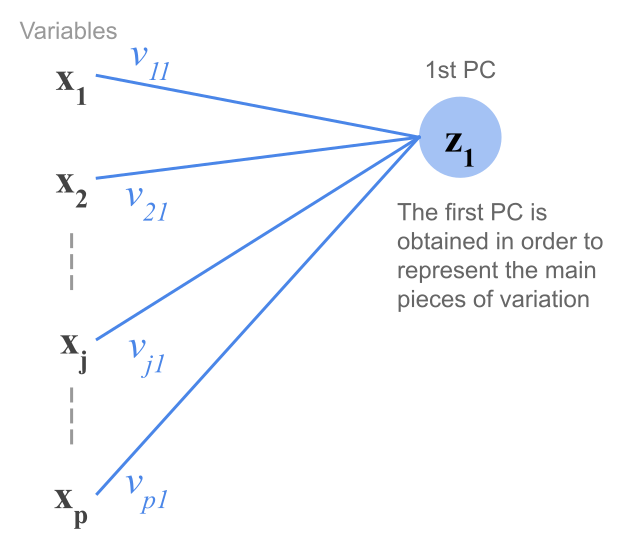
\includegraphics[width=0.5\linewidth]{images/pca/pca-path-diag1} 

}

\caption{PCs as linear combinations of X-variables}\label{fig:unnamed-chunk-27}
\end{figure}

The second PC is another linear mix:

\begin{figure}

{\centering 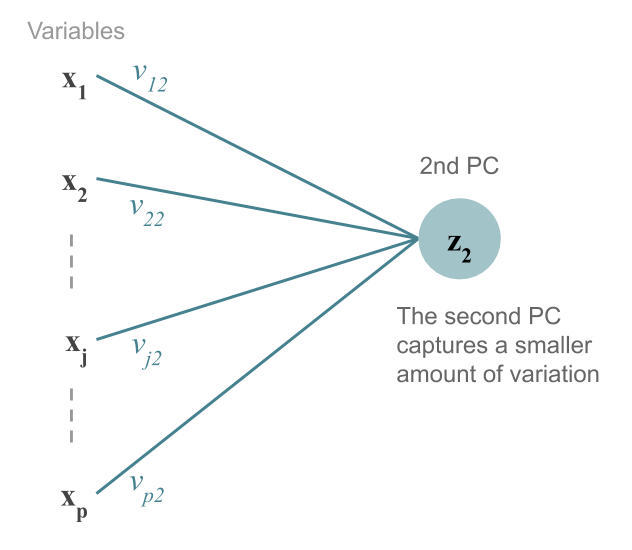
\includegraphics[width=0.5\linewidth]{images/pca/pca-path-diag2} 

}

\caption{PCs as linear combinations of X-variables}\label{fig:unnamed-chunk-28}
\end{figure}

We want to compute the \textbf{PCs as linear combinations} of the original variables.

\[ 
\begin{array}{c}
\mathbf{z_1} = v_{11} \mathbf{x_1} + \dots + v_{1p} \mathbf{x_p} \\
\mathbf{z_2} = v_{21} \mathbf{x_1} + \dots + v_{2p} \mathbf{x_p} \\
\vdots \\
\mathbf{z_k} = v_{k1} \mathbf{x_1} + \dots + v_{kp} \mathbf{x_p} \\
\end{array}
\]

Or in matrix notation:

\[
\mathbf{Z} = \mathbf{X V}
\]

where \(\mathbf{Z}\) is an \(n \times k\) matrix of principal components, and
\(\mathbf{V}\) is a \(p \times k\) matrix of weights, also known as directional
vectors of the principal axes. The following figure shows a graphical
representation of a PCA problem in diagram notation:

\begin{figure}

{\centering 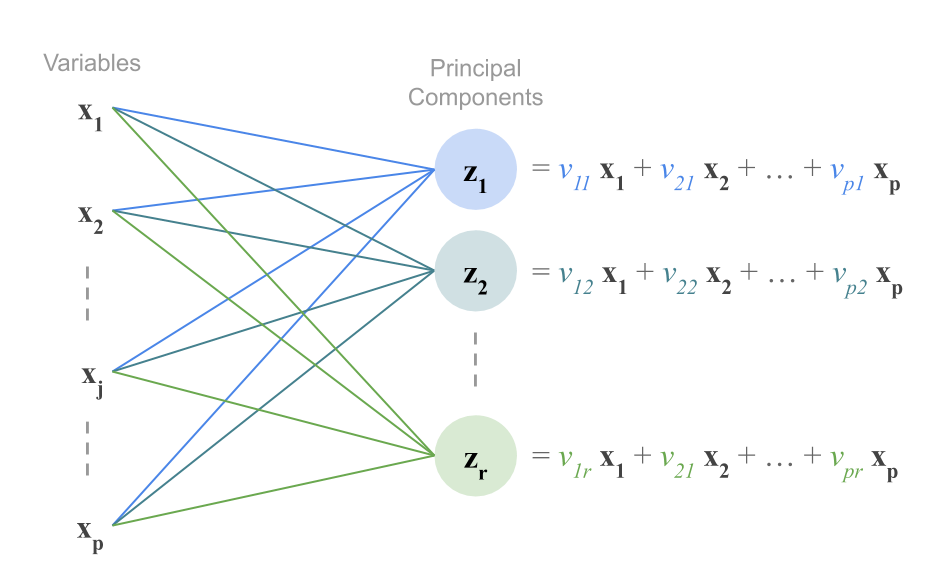
\includegraphics[width=0.7\linewidth]{images/pca/pca-path-diag4} 

}

\caption{PCs as linear combinations of X-variables}\label{fig:unnamed-chunk-29}
\end{figure}

We look to transform the original variables into a smaller set of new variables,
the Principal Components (PCs), that summarize the variation in data.
The PCs are obtained as linear combinations (i.e.~weighted sums) of the
original variables. We look for PCs is in such a way that they have maximum
variance, and being mutually uncorrelated.

\hypertarget{finding-principal-components}{%
\subsection{Finding Principal Components}\label{finding-principal-components}}

The way to find principal components is to construct them as weighted sums of
the original variables, looking to optimize some criterion and following some
constraints. One way in which we can express the criterion is to require components
\(\mathbf{z_1}, \mathbf{z_2}, \dots, \mathbf{z_k}\) that capture most of the variation
in the data \(\mathbf{X}\). ``Capturing most of the variation,'' implies looking
for a vector \(\mathbf{v_j}\) such that a component \(\mathbf{z_h} = \mathbf{X v_h}\)
has maximum variance:

\[
\max_{\mathbf{v_h}} \; var(\mathbf{z_h}) \quad \Rightarrow \quad \max_{\mathbf{v_h}} \; var(\mathbf{X v_h})
\]

that is

\[
\max_{\mathbf{v_h}} \; \frac{1}{n} \mathbf{v_{h}^\mathsf{T} X^\mathsf{T} X v_h}
\]

As you can tell, this is a maximization problem. Without any constraints, this
problem is unbounded, not to mention useless. We could take \(\mathbf{v_h}\) as
bigger as we want without being able to reach any maximum. To get a feasible
solution we need to impose some kind of restriction. The standard adopted
constraint is to require \(\mathbf{v_h}\) to be of unit norm:

\[
\| \mathbf{v_h} \| = 1 \; \hspace{1mm} \Rightarrow \; \hspace{1mm} \mathbf{v_{h}^\mathsf{T} v_h} = 1 
\]

Note that \((1/n) \mathbf{X^\mathsf{T} X}\) is the variance-covariance matrix.
If we denote \(\mathbf{S} = (1/n) \mathbf{X^\mathsf{T} X}\) then the criterion to
be maximized is:

\[
\max_{\mathbf{v_h}} \; \mathbf{v_{h}^\mathsf{T} S v_h}
\]

subject to \(\mathbf{v_{h}^\mathsf{T} v_h} = 1\)

To avoid a PC \(\mathbf{z_h}\) from capturing the same variation as other PCs
\(\mathbf{z_l}\) (i.e.~avoiding redundant information), we also require them to be
\textbf{mutually orthogonal} so they are uncorrelated with each other. Formally,
we impose the restriction \(\mathbf{z_h}\) to be perpendicular to other components:
\(\mathbf{z_{h}^\mathsf{T} z_l} = 0; (h \neq l)\).

\hypertarget{finding-the-first-pc}{%
\subsection{Finding the first PC}\label{finding-the-first-pc}}

In order to get the first principal component \(\mathbf{z_1} = \mathbf{X v_1}\),
we need to find \(\mathbf{v_1}\) such that:

\[
\max_{\mathbf{v_1}} \; \mathbf{v_{1}^\mathsf{T} S v_1}
\]

subject to \(\mathbf{v_{1}^\mathsf{T} v_1} = 1\)

Being a maximization problem, the typical procedure to find the solution is by
using the \textbf{Lagrangian multiplier} method. Using Lagrange multipliers we get:

\[
\mathbf{v_{1}^\mathsf{T} S v_1} - \lambda (\mathbf{v_{1}^\mathsf{T} v_1} - 1) = 0
\]

Differentiation with respect to \(\mathbf{v_1}\), and equating to zero gives:

\[
\mathbf{S v_1} - \lambda_1 \mathbf{v_1} = \mathbf{0}
\]

Rearranging some terms we get:

\[
\mathbf{S v_1} = \lambda_1 \mathbf{v_1}
\]

What does this mean? It means that \(\lambda_1\) is an eigenvalue of \(\mathbf{S}\),
and \(\mathbf{v_1}\) is the corresponding eigenvector.

\hypertarget{finding-the-second-pc}{%
\subsection{Finding the second PC}\label{finding-the-second-pc}}

In order to find the second principal component \(\mathbf{z_2} = \mathbf{X v_2}\),
we need to find \(\mathbf{v_2}\) such that

\[
\max_{\mathbf{v_2}} \; \mathbf{v_{2}^\mathsf{T} S v_2}
\]

subject to \(\| \mathbf{v_2} \| = 1\) and \(\mathbf{z_{1}^\mathsf{T} z_2} = 0\).
Remember that \(\mathbf{z_2}\) must be uncorrelated to \(\mathbf{z_1}\).
Applying the Lagrange multipliers, it can be shown that the desired
\(\mathbf{v_2}\) is such that

\[
\mathbf{S v_2} = \lambda_2 \mathbf{v_2}
\]

In other words. \(\lambda_2\) is an eigenvalue of \(\mathbf{S}\) and \(\mathbf{v_2}\)
is the corresponding eigenvector.

\hypertarget{finding-all-pcs}{%
\subsection{Finding all PCs}\label{finding-all-pcs}}

All PCs can be found simultaneously by \textbf{diagonalizing} \(\mathbf{S}\).
Diagonalizing \(\mathbf{S}\) involves expressing it as the product:

\[ 
\mathbf{S} = \mathbf{V \Lambda V^\mathsf{T}}
\]

where:

\begin{itemize}
\tightlist
\item
  \(\mathbf{D}\) is a diagonal matrix
\item
  the elements in the diagonal of \(\mathbf{D}\) are the eigenvalues of \(\mathbf{S}\)
\item
  the columns of \(\mathbf{V}\) are orthonormal: \(\mathbf{V^\mathsf{T} V= I}\)
\item
  the columns of \(\mathbf{V}\) are the eigenvectors of \(\mathbf{S}\)
\item
  \(\mathbf{V^\mathsf{T}} = \mathbf{V^{-1}}\)
\end{itemize}

Diagonalizing a symmetric matrix is nothing more than obtaining its
\textbf{eigenvalue decomposition} (a.k.a. spectral decomposition).
A \(p \times p\) symmetric matrix \(\mathbf{S}\) has the following properties:

\begin{itemize}
\tightlist
\item
  \(\mathbf{S}\) has \(p\) real eigenvalues (counting multiplicites)
\item
  the eigenvectors corresponding to different eigenvalues are orthogonal
\item
  \(\mathbf{S}\) is orthogonally diagonalizable (\(\mathbf{S} = \mathbf{V \Lambda V^\mathsf{T}}\))
\item
  the set of eigenvalues of \(\mathbf{S}\) is called the \textbf{spectrum} of \(\mathbf{S}\)
\end{itemize}

In summary: The PCA solution can be obtained with an Eigenvalue Decomposition
of the matrix \(\mathbf{S} = (1/n) \mathbf{X^\mathsf{T}X}\)

\hypertarget{pca-model}{%
\section{PCA Model}\label{pca-model}}

Formally, PCA involves finding scores and loadings such that the data can be
expressed as a product of two matrices:

\[
\underset{n \times p}{\mathbf{X}} = \underset{n \times k}{\mathbf{Z}} \underset{k \times p}{\mathbf{V^\mathsf{T}}}
\]

where \(\mathbf{Z}\) is the matrix of PCs or \emph{scores}, and \(\mathbf{V}\) is the
matrix of \emph{loadings}. We can obtain as many different eigenvalues as the rank of
\(\mathbf{S}\) denoted by \(k\). Ideally, we expect \(k\) to be smaller than \(p\)
so we get a convenient data reduction. But usually we will only retain just a
few PCs (i.e.~\(k \ll p\)) expecting not to lose too much information:

\[
\underset{n \times p}{\mathbf{X}} \approx \underset{n \times k}{\mathbf{Z}} \hspace{1mm} \underset{k \times p}{\mathbf{V^\mathsf{T}}} + \text{Residual}
\]

The previous expression means that just a few PCs will \emph{optimally} summarize the main structure of the data

\hypertarget{another-perspective}{%
\section{Another Perspective}\label{another-perspective}}

Finding \(\mathbf{z_h} = \mathbf{X v_h}\) with maximum variance has another
important property that it is not always mentioned in multivariate textbooks
but that we find worth mentioning. \(\mathbf{z_h}\) is such that

\[
\max \sum_{j = 1}^{p} cor^2(\mathbf{z_h, x_j})
\]

What this expression implies is that principal components \(\mathbf{z_h}\) are
computed to be the \emph{best} representants in terms of maximizing the sum of
squared correlations with the variables
\(\mathbf{x_1}, \mathbf{x_2}, \dots, \mathbf{x_j}\).
Interestingly, you can think of PCs as predictors
of the variables in \(\mathbf{X}\). Under this perspective, we can reverse the
relations and see PCA from a regression-like model perspective:

\[
\mathbf{x_j} = v_{jh} \mathbf{z_h} + \mathbf{e_h}
\]

Notice that the regression coefficient is the \(j\)-th element of the \(h\)-th
eigenvector.

\bibliography{book.bib,packages.bib}


\end{document}
